\section{Method}
\label{sec:method}
VADD learns action representations from demonstrations and trains an
editor to execute them under source conditioning
(Figure~\ref{fig:vadd-method}). The editor receives source $V_{\mathrm s}$,
instruction $i$, and demonstration $V_{\mathrm r}$, any video that performs
the requested action, such as a reference recording or a text-to-video
sample; it need not share the source's appearance or frame alignment.
Section~\ref{subsec:experimental-setup} describes the demonstrations used
in training and at inference.

\begin{figure}[!t]
 \centering
 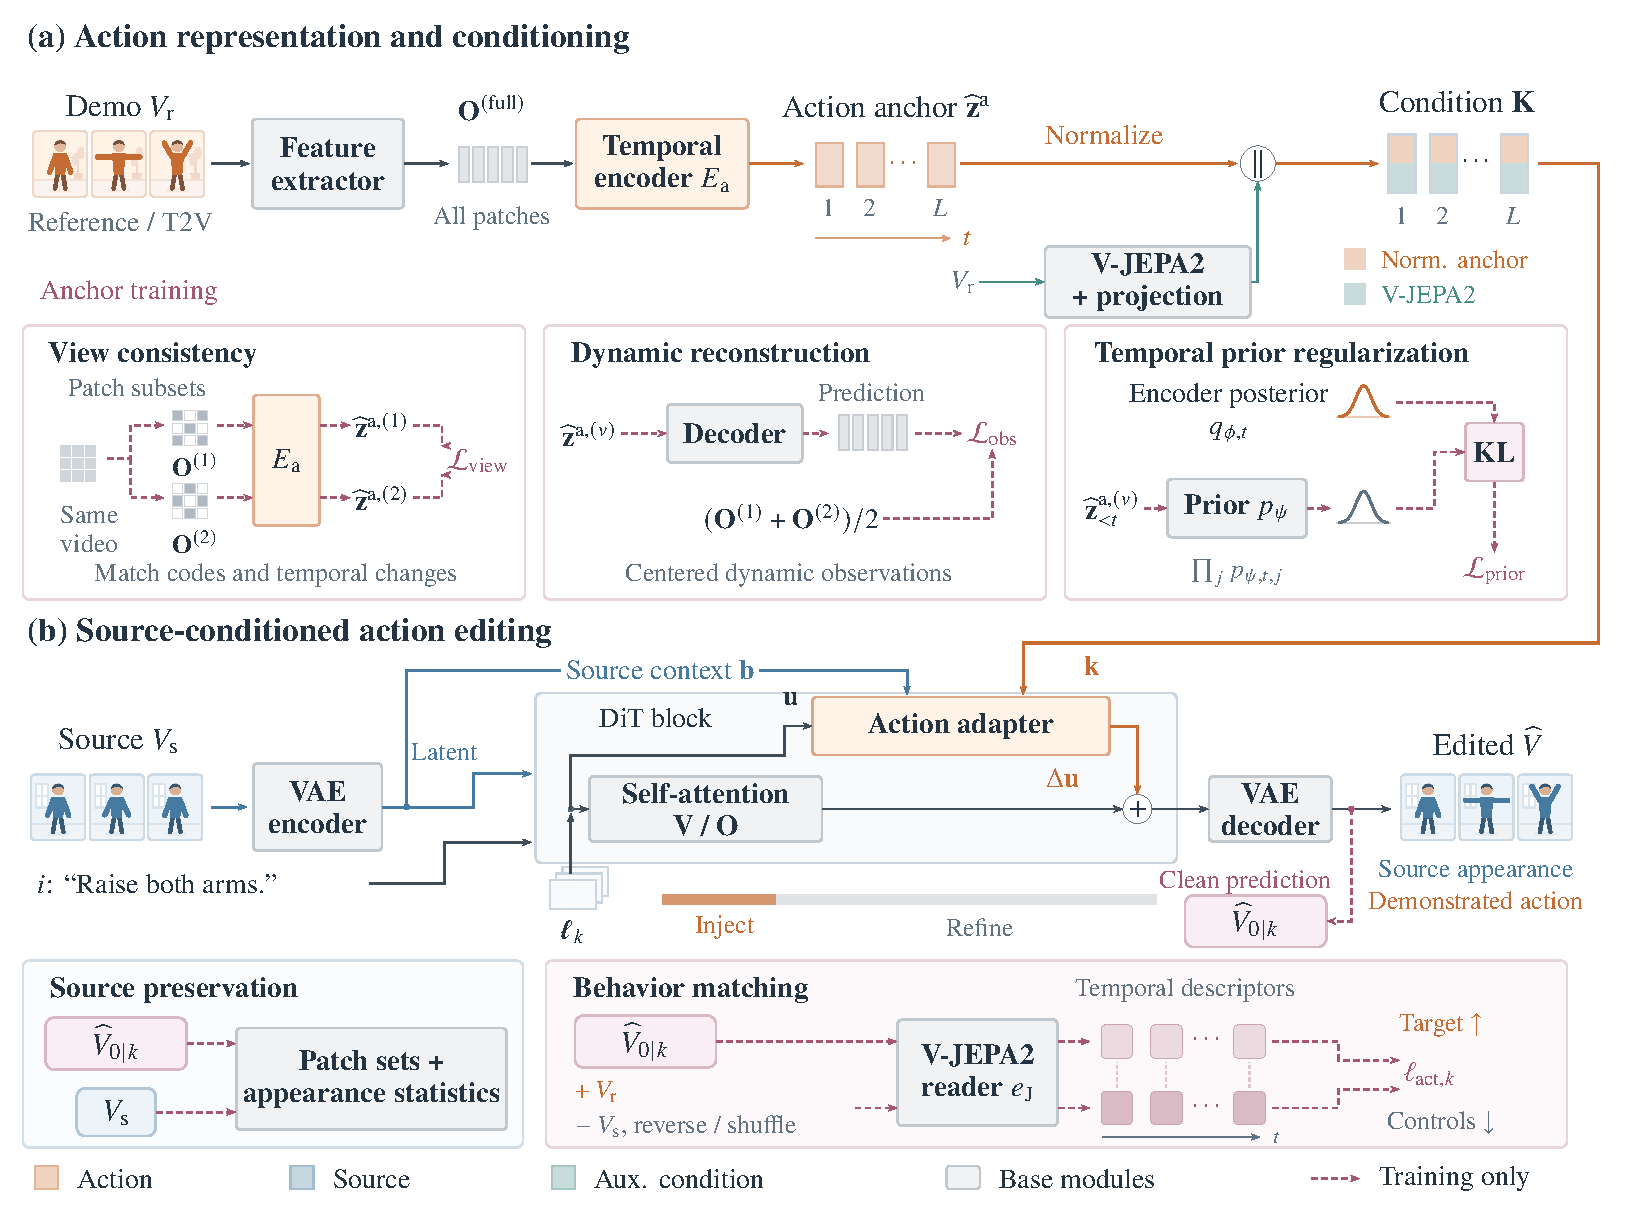
\includegraphics[width=\linewidth]{vadd_method_overview_anchor.pdf}
 \caption{VADD overview.
 (a) A temporal encoder extracts action anchors from full dynamic observations.
 Normalized anchors (orange) and compressed V-JEPA2 features (teal) form
 $\mathbf K$. Training uses same-video patch views for consistency,
 dynamic-observation reconstruction, and KL matching to a history-conditioned
 factorized prior.
 (b) Source context, generated states, and phase-aligned action conditions
 drive residual adapters during early sampling steps.
 Clean predictions receive source-preservation and ordered behavior
 supervision, with source, reversed, and shuffled videos as controls.
 Dashed paths denote training; repeated $\widehat V_{0\mid k}$ ports refer
 to the same prediction. Source/text preprocessing and the sampling loop
 are condensed. Videos, tokens, and distributions are schematic.}
 \label{fig:vadd-method}
\end{figure}

\subsection{Learning action representations from demonstrations}
\label{subsec:method-anchor}

Frozen backbone features of a demonstration yield dynamic observations $\mathbf O(V_{\mathrm r})\in\R^{L\times d_o}$ over $L$
resampled temporal phases. Temporal centering removes constant offsets;
signed changes and local change magnitudes retain direction and variation.
Alternating spatial patches of the same video provide two training views.

A bidirectional recurrent encoder produces a Gaussian posterior
$q_\phi(\widetilde{\mathbf z}^{\mathrm a}_{1:L}\mid \mathbf O)$. Its mean sequence $\widehat{\mathbf z}^{\mathrm a}=E_{\mathrm a}(V_{\mathrm r})=\boldsymbol\mu_\phi(\mathbf O(V_{\mathrm r}))$ serves as the
learned action anchor, with $d_{\mathrm a}=Ld_z$ after vectorization. A history-conditioned prior factorizes as
\begin{equation}
 p_\psi(\widetilde{\mathbf z}^{\mathrm a}_{1:L})
 =\prod_{t=1}^{L}\prod_{j=1}^{d_z}
   p_{\psi,t,j}(\widetilde z^{\mathrm a}_{t,j}\mid \widetilde{\mathbf z}^{\mathrm a}_{<t}),\qquad \widetilde{\mathbf z}^{\mathrm a}_t\in\R^{d_z}.
 \label{eq:method-action-prior}
\end{equation}
Each Gaussian factor's mean depends on preceding latent states through a
shared recurrent state. We evaluate the recurrent decoder and prior on
posterior means and train the representation model with
\begin{equation}
 \mathcal L_{\mathrm{anchor}}
 =\lambda_{\mathrm{obs}}\mathcal L_{\mathrm{obs}}
  +\lambda_{\mathrm{view}}\mathcal L_{\mathrm{view}}
  +\mathcal L_{\mathrm{reg}}.
 \label{eq:method-anchor-loss}
\end{equation}
Here $\mathcal L_{\mathrm{obs}}$ reconstructs the two views' centered mean
observation with SmoothL1, while $\mathcal L_{\mathrm{view}}$ aligns centered
codes and temporal changes. The grouped regularizer $\mathcal L_{\mathrm{reg}}$
combines prior matching, temporal penalties, and discrimination against
reversed, shuffled, and repeated-frame controls. These terms promote
action retention and view invariance.

These objectives follow the invariance and information-retention principles
of Eq.~\ref{eq:anchor-objective}. Shared-scene patch views and mean-target
SmoothL1 prediction are practical surrogates for independent appearance
resampling and distribution prediction, rather than an implementation of
the characteristic-kernel criterion
(Appendix~\ref{subsec:conditioning-proof}).
The recurrent prior supplies temporal inductive bias.

\subsection{Source-conditioned action injection}
\label{subsec:method-editing}

The identification criterion in Definition~\ref{def:anchor-identification}
concerns the learned mean code. The editor receives an augmented condition:
the normalized code concatenated with compressed, ordered V-JEPA2 features
$\Psi_{\mathrm J}(V_{\mathrm r})$~\citep{assran2025vjepa2}:
\begin{equation}
 \mathbf K(V_{\mathrm r})=\operatorname{stopgrad}\!\left(
  \operatorname{Concat}_{\mathrm{feat}}\!\left[
    \operatorname{Norm}_{\mathrm{phase}}(\widehat{\mathbf z}^{\mathrm a}),
    \Psi_{\mathrm J}(V_{\mathrm r})\right]\right).
 \label{eq:method-action-condition}
\end{equation}
The source supplies its video latent and spatial context
$\mathbf b=b_{\mathrm{src}}(V_{\mathrm s})$ from independently encoded frames; the instruction
uses the backbone's text-conditioning path.

Low-rank adapters~\citep{hu2022lora} inject the action into visual
self-attention value and output projections. For generated token $\mathbf u$, phase-aligned row $\mathbf k$ of $\mathbf K$, and source context $\mathbf b$, the update is
\begin{equation}
 \Delta \mathbf u=\alpha_k \mathbf W_{\mathrm{up}}\!\left[
  (\mathbf W_u \mathbf u)\odot\tanh(\mathbf W_k \mathbf k)
  +(\mathbf W_k \mathbf k)\odot\bigl(\mathbf 1+\tanh(\mathbf W_b \mathbf b)\bigr)\right].
 \label{eq:method-adapter}
\end{equation}
The two terms couple the action to the generated state and source context,
respectively. At sampling step $k$, $\alpha_k$ gates action injection;
only early steps use the adapters, with later refinement left to the backbone.

\subsection{Training the editor and inference}
\label{subsec:method-training}

We freeze the representation model and video backbone and train the
adapters. Following a warm-up with action-code alignment, we supervise
output video behavior. At selected early sampling steps $k$, we decode the model's
current clean-video estimate $\widehat V_{0\mid k}$ and compare its motion
with the demonstration through a frozen V-JEPA2 reader $e_{\mathrm J}$.
This reader supplies output supervision separately from the compressed
conditioning branch. Let
$\gamma_{j,k}=\operatorname{sim}(e_{\mathrm J}(\widehat V_{0\mid k}),e_{\mathrm J}(V_j))$
be the mean cosine similarity of ordered descriptors, with
$\mathcal K=\{+,\mathrm{src},\mathrm{rev},\mathrm{shuf}\}$ indexing the
demonstration, source, reversed demonstration, and shuffled demonstration.
The behavior loss
\begin{equation}
 \ell_{\mathrm{act},k}=1-\gamma_{+,k}
  -\lambda_{\mathrm{disc}}\log
   \frac{\exp(\gamma_{+,k}/\tau)}
        {\sum_{j\in\mathcal K}\exp(\gamma_{j,k}/\tau)}
 \label{eq:method-behavior-loss}
\end{equation}
attracts the output toward the demonstrated motion and discriminates it
from source behavior and temporal controls. Gradients pass through the
reader on generated videos; reference descriptors are detached.

Source preservation compares patch sets and appearance statistics.
We remove the component of its gradient that opposes the behavior gradient
in clean-prediction space, then cap its RMS relative to the behavior gradient.
Appendix~\ref{subsec:impl-editing-evidence} specifies the training queries,
preservation rule, and sampling configuration.
Inference extracts $\mathbf K(V_{\mathrm r})$ once and runs the conditional
sampler, without behavior-reader gradients or per-example optimization.
